\documentclass[main.tex]{subfiles}
\begin{document}
\begin{frame}[c]

	\large Ukuran Nilai Sentral :\\
	\Large Rata-rata

\end{frame}

\begin{frame}[c]
	\frametitle{Macam-Macam Nilai Sentral}
	\begin{itemize}
		\item Rata-rata
		\item Median
		\item Mode
		\item Rata-rata ukur
		\item Rata-rata harmoni
		\item Rata-rata Kuadrat
	\end{itemize}
\end{frame}

\begin{frame}[c]
	\frametitle{Rata-rata Hitung (Arithmatic Mean)}
	\textcolor{blue}{Rata-rata merupakan} hasil bagi dari sejumlah nilai dengan banyaknya responden atau sample. Perhitungan mean merupakan perhitungan yang sederhan, karena hanya \textcolor{green}{ membutuhkan jumlah nilai dan jumlah responden (n).}

	Jika sebaran \textit{nilai berdistribusi normal}, maka rata-rata nilai merupakan \textcolor{blue}{nilai tengah} dari distribusi frekuensi nilai tersebut.

	Rata-rata dalam suatu rangkaian data adalah \textcolor{blue}{jumlah seluruh data} dibagi dengan \textit{seluruh kejadian.}
\end{frame}

\begin{frame}[c]
	\frametitle{Rata-rata Hitung (Arithmatic Mean)}
	\framesubtitle{subtitle}
	\begin{center}
		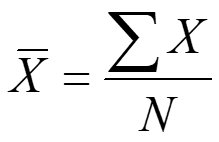
\includegraphics[scale=.5]{figures/mean1}
	\end{center}

	= X bar yang merupakan notasi rata-rata\\
	= Sigma = jumlah\\
	X = nilai dari keseluruhan data\\
	N = jumlah data\\
\end{frame}
\begin{frame}[c]
	\frametitle{Rata-rata Hitung (Arithmatic Mean)}
	Berikut ini adalah \textcolor{blue}{jumlah saudara kandung} dari 5 mahasiswa yang dipilih secara acak, \textit{yaitu ; 2; 4; 6; 8; 10.}

	Maka rata-rata jumlah saudara kandung ke-5 mahasiswa tersebut adalah

	\begin{center}
		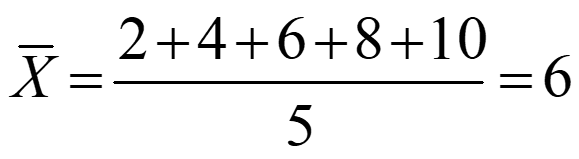
\includegraphics[scale=0.5]{figures/mean2}
	\end{center}


\end{frame}

\begin{frame}[c]
	\frametitle{Rata-rata Hitung (Arithmatic Mean)}

	Apabila data yang ada sudah {\Large dikelompokkan} ke dalam distribusi frekuensi, maka cara perhitungan adalah sebagai berikut :

	Cari Nilai tengah untuk setiap kelas

	Kalikan nilai tengah dengan frekuensi

	Hitung rata-rata dengan menggunakan rumus

	\begin{center}
		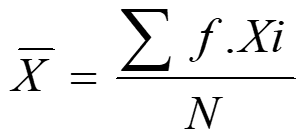
\includegraphics[scale=.5]{figures/mean3}
	\end{center}
\end{frame}

\begin{frame}[c]
	\frametitle{Rata-rata Hitung (Arithmatic Mean)}
	\small
	\begin{table}[htb]
		\begin{tabular}{p{1.5cm}p{1.5cm}p{1.5cm}p{1.5cm}}
			\hline
			Gaji karyawan (kelas)  &  Jumlah karyawan  &  Nilai Tengah  &  Frekuensi x Nilai tengah  \\
			\hline
			30-39                  &  4                &  34.5          &  138  \\
			40-49                  &  6                &  44.5          &  267  \\
			50-59                  &  8                &  54.5          &  436  \\
			60-69                  &  12               &  64.5          &  774  \\
			70-79                  &  9                &  74.5          &  670.5  \\
			80-89                  &  7                &  84.5          &  591.5  \\
			90-99                  &  4                &  94.5          &  378  \\
			\hline
			                       &  N= 50            &                &  3255  \\
		\end{tabular}
	\end{table}
	\begin{textblock*}{2cm}(9cm,7cm) % {block width} (coords.12,8cm)
		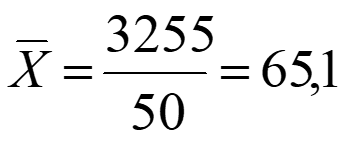
\includegraphics[width=3cm]{figures/mean4}
	\end{textblock*}

\end{frame}

\begin{frame}[c]
	\frametitle{Rata-Rata Ukur}
	Rata-rata ukur adalah akar pangkat n dari hasil perkalian datanya

	\begin{center}
		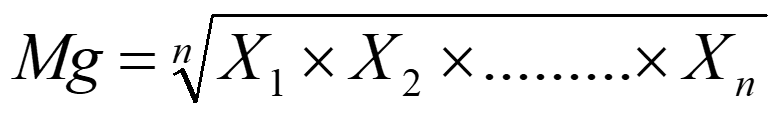
\includegraphics[scale=.5]{figures/mean5}
	\end{center}
\end{frame}

\begin{frame}[c]
	\frametitle{Rata-rata Harmoni}
	Rata-rata harmoni adalah kebalikan dari rata-rata hitung

	\begin{center}
		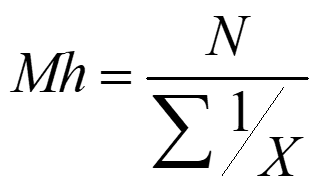
\includegraphics[scale=.5]{figures/mean6}
	\end{center}

\end{frame}

\begin{frame}[c]
	\frametitle{Rata-rata Kuadrat}
	Rata-rata kuadrat adalah akar pangkat dua dari kuadrat nilai rata-ratanya

	\begin{center}
		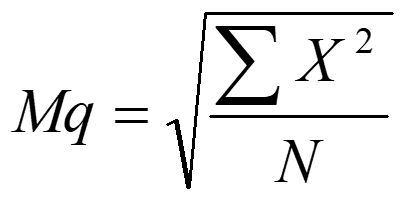
\includegraphics[scale=.5]{figures/mean7}
	\end{center}

\end{frame}


\end{document}

